
%% bare_conf.tex
%% V1.4b
%% 2015/08/26
%% by Michael Shell
%% See:
%% http://www.michaelshell.org/
%% for current contact information.
%%
%% This is a skeleton file demonstrating the use of IEEEtran.cls
%% (requires IEEEtran.cls version 1.8b or later) with an IEEE
%% conference paper.
%%
%% Support sites:
%% http://www.michaelshell.org/tex/ieeetran/
%% http://www.ctan.org/pkg/ieeetran
%% and
%% http://www.ieee.org/

%%*************************************************************************
%% Legal Notice:
%% This code is offered as-is without any warranty either expressed or
%% implied; without even the implied warranty of MERCHANTABILITY or
%% FITNESS FOR A PARTICULAR PURPOSE! 
%% User assumes all risk.
%% In no event shall the IEEE or any contributor to this code be liable for
%% any damages or losses, including, but not limited to, incidental,
%% consequential, or any other damages, resulting from the use or misuse
%% of any information contained here.
%%
%% All comments are the opinions of their respective authors and are not
%% necessarily endorsed by the IEEE.
%%
%% This work is distributed under the LaTeX Project Public License (LPPL)
%% ( http://www.latex-project.org/ ) version 1.3, and may be freely used,
%% distributed and modified. A copy of the LPPL, version 1.3, is included
%% in the base LaTeX documentation of all distributions of LaTeX released
%% 2003/12/01 or later.
%% Retain all contribution notices and credits.
%% ** Modified files should be clearly indicated as such, including  **
%% ** renaming them and changing author support contact information. **
%%*************************************************************************


% *** Authors should verify (and, if needed, correct) their LaTeX system  ***
% *** with the testflow diagnostic prior to trusting their LaTeX platform ***
% *** with production work. The IEEE's font choices and paper sizes can   ***
% *** trigger bugs that do not appear when using other class files.       ***                          ***
% The testflow support page is at:
% http://www.michaelshell.org/tex/testflow/



\documentclass[conference]{IEEEtran}
% Some Computer Society conferences also require the compsoc mode option,
% but others use the standard conference format.
%
% If IEEEtran.cls has not been installed into the LaTeX system files,
% manually specify the path to it like:
% \documentclass[conference]{../sty/IEEEtran}





% Some very useful LaTeX packages include:
% (uncomment the ones you want to load)


% *** MISC UTILITY PACKAGES ***
%
%\usepackage{ifpdf}
% Heiko Oberdiek's ifpdf.sty is very useful if you need conditional
% compilation based on whether the output is pdf or dvi.
% usage:
% \ifpdf
%   % pdf code
% \else
%   % dvi code
% \fi
% The latest version of ifpdf.sty can be obtained from:
% http://www.ctan.org/pkg/ifpdf
% Also, note that IEEEtran.cls V1.7 and later provides a builtin
% \ifCLASSINFOpdf conditional that works the same way.
% When switching from latex to pdflatex and vice-versa, the compiler may
% have to be run twice to clear warning/error messages.



\usepackage{float}
\usepackage{booktabs}
\usepackage{algorithmic}
\usepackage{algorithm2e}
\usepackage{listings}
\usepackage{float}
\usepackage{color}

% *** CITATION PACKAGES ***
%
\usepackage{cite}
% cite.sty was written by Donald Arseneau
% V1.6 and later of IEEEtran pre-defines the format of the cite.sty package
% \cite{} output to follow that of the IEEE. Loading the cite package will
% result in citation numbers being automatically sorted and properly
% "compressed/ranged". e.g., [1], [9], [2], [7], [5], [6] without using
% cite.sty will become [1], [2], [5]--[7], [9] using cite.sty. cite.sty's
% \cite will automatically add leading space, if needed. Use cite.sty's
% noadjust option (cite.sty V3.8 and later) if you want to turn this off
% such as if a citation ever needs to be enclosed in parenthesis.
% cite.sty is already installed on most LaTeX systems. Be sure and use
% version 5.0 (2009-03-20) and later if using hyperref.sty.
% The latest version can be obtained at:
% http://www.ctan.org/pkg/cite
% The documentation is contained in the cite.sty file itself.






% *** GRAPHICS RELATED PACKAGES ***
%
\ifCLASSINFOpdf
  \usepackage[pdftex]{graphicx}
  % declare the path(s) where your graphic files are
  % \graphicspath{{../pdf/}{../jpeg/}}
  % and their extensions so you won't have to specify these with
  % every instance of \includegraphics
  % \DeclareGraphicsExtensions{.pdf,.jpeg,.png}
\else
  % or other class option (dvipsone, dvipdf, if not using dvips). graphicx
  % will default to the driver specified in the system graphics.cfg if no
  % driver is specified.
  \usepackage[dvips]{graphicx}
  % declare the path(s) where your graphic files are
  % \graphicspath{{../eps/}}
  % and their extensions so you won't have to specify these with
  % every instance of \includegraphics
  % \DeclareGraphicsExtensions{.eps}
\fi
% graphicx was written by David Carlisle and Sebastian Rahtz. It is
% required if you want graphics, photos, etc. graphicx.sty is already
% installed on most LaTeX systems. The latest version and documentation
% can be obtained at: 
% http://www.ctan.org/pkg/graphicx
% Another good source of documentation is "Using Imported Graphics in
% LaTeX2e" by Keith Reckdahl which can be found at:
% http://www.ctan.org/pkg/epslatex
%
% latex, and pdflatex in dvi mode, support graphics in encapsulated
% postscript (.eps) format. pdflatex in pdf mode supports graphics
% in .pdf, .jpeg, .png and .mps (metapost) formats. Users should ensure
% that all non-photo figures use a vector format (.eps, .pdf, .mps) and
% not a bitmapped formats (.jpeg, .png). The IEEE frowns on bitmapped formats
% which can result in "jaggedy"/blurry rendering of lines and letters as
% well as large increases in file sizes.
%
% You can find documentation about the pdfTeX application at:
% http://www.tug.org/applications/pdftex





% *** MATH PACKAGES ***
%
\usepackage{amsmath}
% A popular package from the American Mathematical Society that provides
% many useful and powerful commands for dealing with mathematics.
%
% Note that the amsmath package sets \interdisplaylinepenalty to 10000
% thus preventing page breaks from occurring within multiline equations. Use:
%\interdisplaylinepenalty=2500
% after loading amsmath to restore such page breaks as IEEEtran.cls normally
% does. amsmath.sty is already installed on most LaTeX systems. The latest
% version and documentation can be obtained at:
% http://www.ctan.org/pkg/amsmath





% *** SPECIALIZED LIST PACKAGES ***
%
%\usepackage{algorithmic}
% algorithmic.sty was written by Peter Williams and Rogerio Brito.
% This package provides an algorithmic environment fo describing algorithms.
% You can use the algorithmic environment in-text or within a figure
% environment to provide for a floating algorithm. Do NOT use the algorithm
% floating environment provided by algorithm.sty (by the same authors) or
% algorithm2e.sty (by Christophe Fiorio) as the IEEE does not use dedicated
% algorithm float types and packages that provide these will not provide
% correct IEEE style captions. The latest version and documentation of
% algorithmic.sty can be obtained at:
% http://www.ctan.org/pkg/algorithms
% Also of interest may be the (relatively newer and more customizable)
% algorithmicx.sty package by Szasz Janos:
% http://www.ctan.org/pkg/algorithmicx




% *** ALIGNMENT PACKAGES ***
%
%\usepackage{array}
% Frank Mittelbach's and David Carlisle's array.sty patches and improves
% the standard LaTeX2e array and tabular environments to provide better
% appearance and additional user controls. As the default LaTeX2e table
% generation code is lacking to the point of almost being broken with
% respect to the quality of the end results, all users are strongly
% advised to use an enhanced (at the very least that provided by array.sty)
% set of table tools. array.sty is already installed on most systems. The
% latest version and documentation can be obtained at:
% http://www.ctan.org/pkg/array


% IEEEtran contains the IEEEeqnarray family of commands that can be used to
% generate multiline equations as well as matrices, tables, etc., of high
% quality.




% *** SUBFIGURE PACKAGES ***
\ifCLASSOPTIONcompsoc
  \usepackage[caption=false,font=normalsize,labelfont=sf,textfont=sf]{subfig}
\else
  \usepackage[caption=false,font=footnotesize]{subfig}
\fi
% subfig.sty, written by Steven Douglas Cochran, is the modern replacement
% for subfigure.sty, the latter of which is no longer maintained and is
% incompatible with some LaTeX packages including fixltx2e. However,
% subfig.sty requires and automatically loads Axel Sommerfeldt's caption.sty
% which will override IEEEtran.cls' handling of captions and this will result
% in non-IEEE style figure/table captions. To prevent this problem, be sure
% and invoke subfig.sty's "caption=false" package option (available since
% subfig.sty version 1.3, 2005/06/28) as this is will preserve IEEEtran.cls
% handling of captions.
% Note that the Computer Society format requires a larger sans serif font
% than the serif footnote size font used in traditional IEEE formatting
% and thus the need to invoke different subfig.sty package options depending
% on whether compsoc mode has been enabled.
%
% The latest version and documentation of subfig.sty can be obtained at:
% http://www.ctan.org/pkg/subfig




% *** FLOAT PACKAGES ***
%
%\usepackage{fixltx2e}
% fixltx2e, the successor to the earlier fix2col.sty, was written by
% Frank Mittelbach and David Carlisle. This package corrects a few problems
% in the LaTeX2e kernel, the most notable of which is that in current
% LaTeX2e releases, the ordering of single and double column floats is not
% guaranteed to be preserved. Thus, an unpatched LaTeX2e can allow a
% single column figure to be placed prior to an earlier double column
% figure.
% Be aware that LaTeX2e kernels dated 2015 and later have fixltx2e.sty's
% corrections already built into the system in which case a warning will
% be issued if an attempt is made to load fixltx2e.sty as it is no longer
% needed.
% The latest version and documentation can be found at:
% http://www.ctan.org/pkg/fixltx2e


%\usepackage{stfloats}
% stfloats.sty was written by Sigitas Tolusis. This package gives LaTeX2e
% the ability to do double column floats at the bottom of the page as well
% as the top. (e.g., "\begin{figure*}[!b]" is not normally possible in
% LaTeX2e). It also provides a command:
%\fnbelowfloat
% to enable the placement of footnotes below bottom floats (the standard
% LaTeX2e kernel puts them above bottom floats). This is an invasive package
% which rewrites many portions of the LaTeX2e float routines. It may not work
% with other packages that modify the LaTeX2e float routines. The latest
% version and documentation can be obtained at:
% http://www.ctan.org/pkg/stfloats
% Do not use the stfloats baselinefloat ability as the IEEE does not allow
% \baselineskip to stretch. Authors submitting work to the IEEE should note
% that the IEEE rarely uses double column equations and that authors should try
% to avoid such use. Do not be tempted to use the cuted.sty or midfloat.sty
% packages (also by Sigitas Tolusis) as the IEEE does not format its papers in
% such ways.
% Do not attempt to use stfloats with fixltx2e as they are incompatible.
% Instead, use Morten Hogholm'a dblfloatfix which combines the features
% of both fixltx2e and stfloats:
%
% \usepackage{dblfloatfix}
% The latest version can be found at:
% http://www.ctan.org/pkg/dblfloatfix




% *** PDF, URL AND HYPERLINK PACKAGES ***
%
\usepackage{url}
% url.sty was written by Donald Arseneau. It provides better support for
% handling and breaking URLs. url.sty is already installed on most LaTeX
% systems. The latest version and documentation can be obtained at:
% http://www.ctan.org/pkg/url
% Basically, \url{my_url_here}.




% *** Do not adjust lengths that control margins, column widths, etc. ***
% *** Do not use packages that alter fonts (such as pslatex).         ***
% There should be no need to do such things with IEEEtran.cls V1.6 and later.
% (Unless specifically asked to do so by the journal or conference you plan
% to submit to, of course. )


% correct bad hyphenation here
\hyphenation{op-tical net-works semi-conduc-tor }

\IEEEoverridecommandlockouts
\begin{document}
%
% paper title
% Titles are generally capitalized except for words such as a, an, and, as,
% at, but, by, for, in, nor, of, on, or, the, to and up, which are usually
% not capitalized unless they are the first or last word of the title.
% Linebreaks \\ can be used within to get better formatting as desired.
% Do not put math or special symbols in the title.
\title{Performance Analysis of Fixed Point Bit Precision for Output Fmaps in CNNs }


% author names and affiliations
% use a multiple column layout for up to three different
% affiliations
%	\author{\IEEEauthorblockN{Michael Shell}
%	\IEEEauthorblockA{School of Electrical and\\Computer Engineering\\
%	Georgia Institute of Technology\\
%	Atlanta, Georgia 30332--0250\\
%	Email: http://www.michaelshell.org/contact.html}
%	\and
%	\IEEEauthorblockN{Homer Simpson}
%	\IEEEauthorblockA{Twentieth Century Fox\\
%	Springfield, USA\\
%	Email: homer@thesimpsons.com}
%	\and
%	\IEEEauthorblockN{James Kirk\\ and Montgomery Scott}
%	\IEEEauthorblockA{Starfleet Academy\\
%	San Francisco, California 96678--2391\\
%	Telephone: (800) 555--1212\\
%	Fax: (888) 555--1212}}

\author{\IEEEauthorblockN{Anaam Ansari\IEEEauthorrefmark{1}\IEEEauthorrefmark{2}\thanks{\IEEEauthorrefmark{2}aaansari@scu.edu}, 
Tokunbo Ogunfunmi\IEEEauthorrefmark{1}\IEEEauthorrefmark{3}\thanks{\IEEEauthorrefmark{3}togunfunmi@scu.edu}}
\IEEEauthorblockA{\IEEEauthorrefmark{1}Department of Electrical Engineering\\
Santa Clara University,
Santa Clara, California 95053}
}


% conference papers do not typically use \thanks and this command
% is locked out in conference mode. If really needed, such as for
% the acknowledgment of grants, issue a \IEEEoverridecommandlockouts
% after \documentclass

% for over three affiliations, or if they all won't fit within the width
% of the page, use this alternative format:
% 
%\author{\IEEEauthorblockN{Michael Shell\IEEEauthorrefmark{1},
%Homer Simpson\IEEEauthorrefmark{2},
%James Kirk\IEEEauthorrefmark{3}, 
%Montgomery Scott\IEEEauthorrefmark{3} and
%Eldon Tyrell\IEEEauthorrefmark{4}}
%\IEEEauthorblockA{\IEEEauthorrefmark{1}School of Electrical and Computer Engineering\\
%Georgia Institute of Technology,
%Atlanta, Georgia 30332--0250\\ Email: see http://www.michaelshell.org/contact.html}
%\IEEEauthorblockA{\IEEEauthorrefmark{2}Twentieth Century Fox, Springfield, USA\\
%Email: homer@thesimpsons.com}
%\IEEEauthorblockA{\IEEEauthorrefmark{3}Starfleet Academy, San Francisco, California 96678-2391\\
%Telephone: (800) 555--1212, Fax: (888) 555--1212}
%\IEEEauthorblockA{\IEEEauthorrefmark{4}Tyrell Inc., 123 Replicant Street, Los Angeles, California 90210--4321}}




% use for special paper notices
%\IEEEspecialpapernotice{(Invited Paper)}




% make the title area
\maketitle

% As a general rule, do not put math, special symbols or citations
% in the abstract
\begin{abstract}
Image classification and speech processing have made Convolutional Neural Networks (CNN) mainstream. Due to their success, many deep networks have been developed such as AlexNet, VGGNet, GoogleNet, ResidualNet \cite{ krizhevsky2012imagenet,he2016deep,szegedy2015going,simonyan2014very},etc. Implementing these deep and complex networks in hardware is a challenge. There have been many hardware and algorithmic solutions to improve the throughput, latency and accuracy. There are many model compression techniques that have been introduced to decrease the model size and help develop a generalized model. Quantization is one such technique. Traditionally, quantized weights and inputs are used  to reduce the memory transfer and power consumption due to it. In this paper, we use quantization on the output of each layer for AlexNet and VGGNET16 and analyze its effect on the soft-max score during forward pass given the prediction is correct. We found that although, there is a deterioration in the softmax confidence score we can lower the bit precision of the output fmap data before suffering a considerable loss. AlexNet performs similarly with single (32 bit) floating point precision and a signed 12 bit fixed point number whereas VGGNET16 using double floating point precision (64 bits) and signed 24 bit fixed point number give a comparable performance. 

\end{abstract}

\begin{IEEEkeywords}
CNN, compressed network, AlexNet, quantization, fixed point.
\end{IEEEkeywords}
% no keywords
% 
% 




% For peer review papers, you can put extra information on the cover
% page as needed:
% 
% 
% \ifCLASSOPTIONpeerreview
% \begin{center} \bfseries EDICS Category: 3-BBND \end{center}
% \fi
%
% For peerreview papers, this IEEEtran command inserts a page break and
% creates the second title. It will be ignored for other modes.
\IEEEpeerreviewmaketitle

%            for w=1:Wout
%                for h=1:Hout
%                    for m=1:M
%                        wStart=(w-1)*S+1;
%                        wEnd=wStart+K-1;
%                        hStart=(h-1)*S+1;
%                        hEnd=hStart+K-1;
%                        top(w,h,m)=top(w,h,m)+sum(sum(sum( ...
%                            bottomPadded(wStart:wEnd,hStart:hEnd,1:N) .* ...
%                            weight(:,:,1:N,m))));
%                    end
%                end

\section{Introduction}
Convolutional Neural Networks are comprised of multiple layers that have different functions. These layers take an input volume and
transform it into an output volume. Successive processing of these layers results in weights that are updated heuristically with each forward pass of input to the output. The operations performed on the input, in a convolutional layer are described in the figure \ref{cnn_ref} \cite{cs231}.
The stages in the covolutional layer are the input stage, the convolutional stage, the non linear stage and the pooling stage. 

The input stage prepares the input volume to be processed by the convolutional stage by conforming it to prescribed dimensions. The prepped input is given to the convolutional stage. This is the stage that does most of the heavy lifting in terms of computational cost such as matrix multiplications and vector multiplications. The convolutional operation is described in algorithm \ref{alg1}. CNNs are neural network that are sparsely connected as they rely on the spatial properties of the input payload. Conventionally, this is the stage where the quantized weights are used. We want to perform fixed point arithmetic and quantize the output 

 There is a nonlinear stage to map the output of the convolutional stage to a continuous limited range. Activation functions are supposed to emulate the generation of `action potential' in a neuron \cite{glorot2011deep}. The purpose of the the activation function is to provide a smooth unique mapping.
 Some of the popular functions used in the non-linear stage are $tanh()$, $sigmoid,$ $\sigma()$ and $relu, max(0,k)$. They are described in the figure \ref{act}. The non linear function $relu$ is used in AlexNet and VGGNET16 as it limits the output to a range $(0,1)$ \cite{ krizhevsky2012imagenet}. 
 
 The maxpooling stage condenses the result of the nonlinear stage into a smaller size. This is akin to down sampling that removes redundant data and makes the processed volume manageable while conserving all the key features and information in it. Pooling converts the output of the net at a certain location to statistics of neighboring outputs. The pooling layer output is invariant to any small translations in the input. This makes the presence of a feature take precedence over th location of the feature \cite{Goodfellow-et-al-2016}
 
This is where we propose the new quantization scheme to lie. We want to assess the quality of performance of the device by quantizing the output of the convolutional layers. 


\begin{figure}[!ht]
\centering
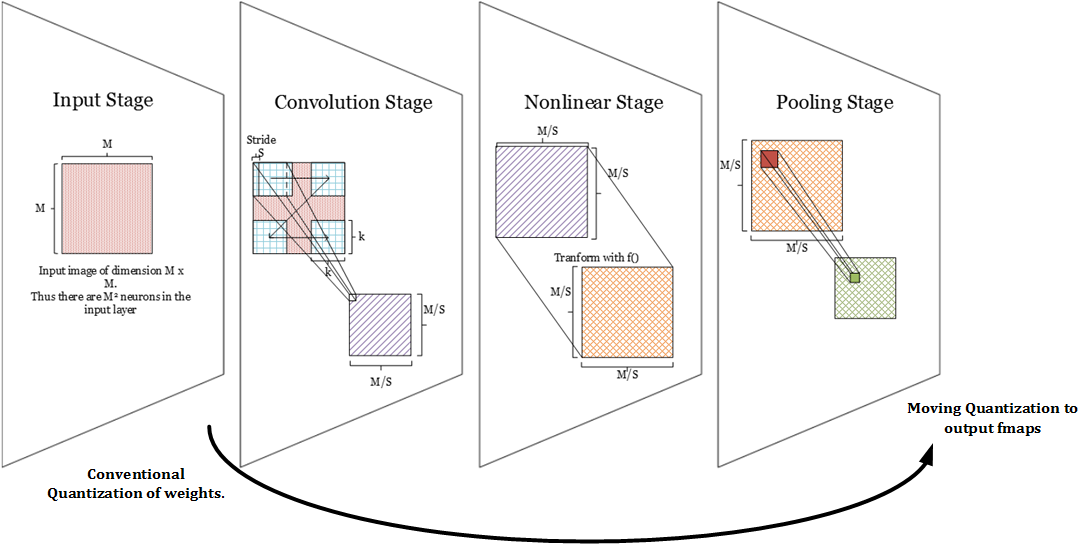
\includegraphics[width=4in]{cnn_trans}
\caption{The functions involved in computing a CNN layer}
\label{cnn_ref}
\end{figure}

A CNN architecture can be organized to have many layers in many combination. The engineering decisions about the depth and size of model can be used to optimize the latency, throughput and accuracy of the network. 


 \begin{figure}[!h]
\centering
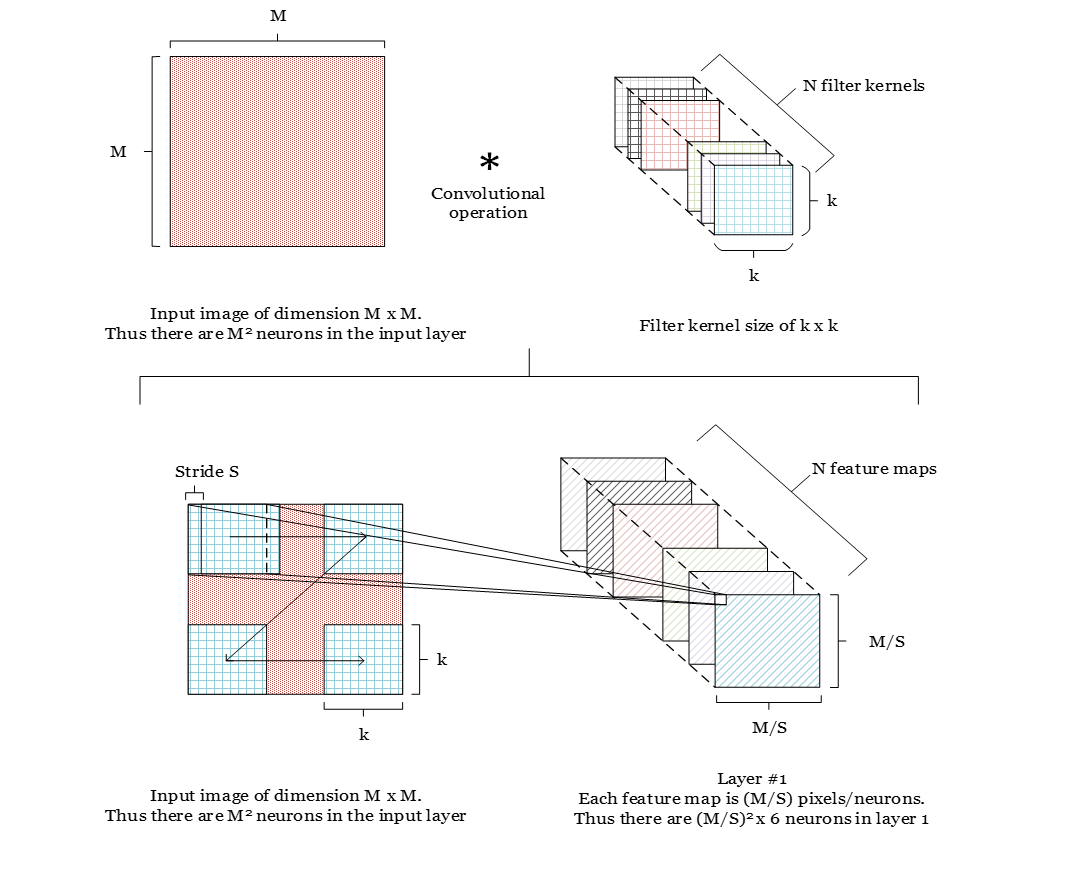
\includegraphics[width=4in]{cnnlayer}
\caption{convolutional operation}
\label{cnn_layer}
\end{figure}



\begin{algorithm}[h!]

\SetKwData{Left}{left}\SetKwData{This}{this}\SetKwData{Up}{up}
\SetKwFunction{Union}{Union}\SetKwFunction{Accumulate}{Accumulate}
\SetKwInOut{Input}{input}\SetKwInOut{Output}{output}

\Input{M inputs, $Imap$ of size $Win\times Hin$}
\Input { Input weights $kernels$ of size $k\times k$}
The stride of the kernels is $S$\\
\Output{$Ofmap$ of size $Wout \times Hout$}
\BlankLine
\SetAlgoLined
\For{($w=0, w<Wout, w++$)}{
\For{($h=0, h<Hout, h++$)}{
\For{($n=0, n<N, n++$)}{

\BlankLine
\small{
$wStart=(w-1)*S+1$;\\
$wEnd=wStart+k-1$;\\
$hStart=(h-1)*S+1$;\\
$hEnd=hStart+k-1$;\\ 
                        $Ofmaps(w,h,n)=$\\
                        $Ofmaps(w,h,n) +$ \\
                      	\Accumulate{\\
                      	\BlankLine
                      	$Imap(wStart:wEnd,hStart:hEnd,1:M)$\\ 
                        $*kernels(:,:,1:M,n))$\\
                        \BlankLine
                        }
                        \BlankLine
              
}    
}

}
}
\caption{2D convolutional operation}
\label{alg1}
\end{algorithm}

 \begin{figure}[!h]
\centering
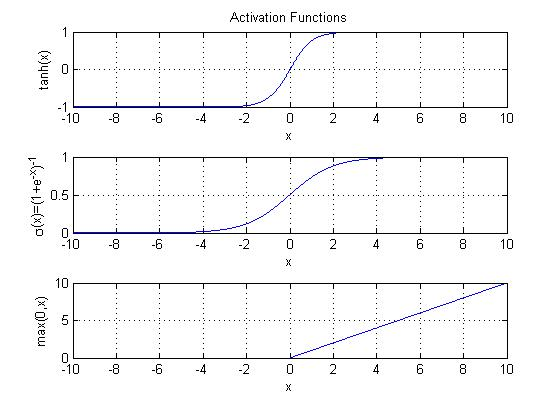
\includegraphics[width=3.5in]{activation}
\caption{Non-linear activation functions}
\label{act}
\end{figure}




\section{ Motivation} 
Techniques like dropout and pruning have been introduced to address problems like overfitting \cite{srivastava2014dropout,zhu2017prune}. They have also helped to compress model sizes. Weight pruning and quantization techniques are used in many hardware devices. 
\cite{han2016eie, jouppi2017datacenter, DBLP:journals/corr/IandolaMAHDK16, jiang2017xnor, tang2017binary}
Works like \textbf{DeepCompression} \cite{han2015deep} have proved that a combination of network optimization techniques such as pruning, quantization and Huffman coding prove very successful in reducing the network size while maintaining accuracy as can be seen in Table \ref{quant_eff}. Most of these techniques are applied to weights since, dense networks are really large and have a large number of parameters. For example AlexNet has about 60M parameters\cite{krizhevsky2012imagenet} and VGGNET16 has 138M \cite{simonyan2014very}. This strategy is valid and will reduce the memory transfer between computation engine and the main memory.

In this paper, we want to explore the effect of quantization in between convolutional layers. We observe the effect of various fixed point bit precisions in the forward path of a network. We examine the results that correctly predict the test image and quantify the \textbf{softmax} score corresponding to a bit precision. A softmax classifier is a generalization of the Logistic Regression Classifier. It defines multiple output classes compared to binary output classes. It takes the input vector and converts it into a normalized vector between 0 and 1 and the sum of that vector is also equal to 1. 

%\begin{equation}
%f_j(z) = \frac{e^{Z_j}}{\Sigma_k e^{z_k}}
%\label{softmax}
%\end{equation}

CNN layers are most often processed iteratively. Thus, the outputs of the CNN layers need to be transported back to memory. As a result, we are interested in 
 reducing the size of the output fmaps. This will help us reduce the memory read and write cycle. Memory transfer for voluminous calculations for convolutional layers and fully-connected layers contributes to a substantial energy consumption and hence power requirement to run the hardware. There are many solutions that address this problem with data reuse and datapath design\cite{Eyeriss,zhang2015optimizing, shen2017escher, shen2017maximizing}. Reducing the amount of output fmaps that need to be written back to memory and read again for the next layer will be helpful in memory transfer reduction. Our work will help contribute to this reduction of memory traffic by quantizing output fmaps into fixed point bit precision


\begin{table*}[h!]
\centering
\caption{Effect of quantization optimization techniques \cite{han2015deep, DBLP:journals/corr/IandolaMAHDK16}}
\label{quant_eff}
\begin{tabular}{cccccc}
\hline
                    & \textbf{Orignial} & \textbf{Compressed } & \textbf{Compression} & \textbf{Original} & \textbf{Compressed} \\ 
\textbf{Network}    & \textbf{Size (MB)}          & \textbf{Size (MB)}            & \textbf{Ratio}             & \textbf{Accuracy} & \textbf{Accuracy}   \\ \hline

\textbf{AlexNet}    & 240                    & 6.9                      & 35x                        & 80.27\%           & 80.30\%             \\
\textbf{VGGNet}     & 550                    & 11.3                     & 49x                        & 88.68\%           & 89.09\%             \\
\textbf{GooglNet}   & 28                     & 2.8                      & 10x                        & 88.90\%           & 88.92\%             \\
\textbf{SqueezeNet} & 4.8                    & 0.47                     & 10x                        & 80.32\%           & 80.35\%             \\ \hline
\end{tabular}
\end{table*}

\section{Networks}
The year 2012 was a momentous year for Deep Learning. The very first Deep Learning entry to the ImageNet challenge \cite{ILSVRC15}  in 2012 was AlexNet \cite{krizhevsky2012imagenet}. It had 60M parameter and was implemented on GPUs. In this paper, we focus on AlexNet  (1st place winner) and VGGNET16 (1st runner up) for the analysis. The analysis can similarly be done for other networks as well.

\subsection{AlexNet}
The overall architecture of AlexNet has 8 layers as seen in figure \ref{fp}. The first five layers are convolutional layers. They perform convolutional operations as described in figure \ref{cnn_layer}. The output of the network is the output of the fully connected layer which is subjected to a softmax probability based classification which can classify an input into  1000 classes. The input to the network is an image of size $227 \times 227 \times 3$ with a fixed stride. The stride is $4$ pixels for AlexNet.
This is operated on by  $96$ filter kernels of size $11 \times 11 \times 3$. The output thus obtained is put through a non-linear $relu$ activation function and maxpooled. The output of the first convolutional layer are $96$ fmaps of size $55 \times 55$. This is acted upon by the second convolutional layer which has $256$ kernels of size $5 \times 5 \times 48$. The third, fourth and fifth convolutional layers act similarly and their kernel sizes and number are described in Table \ref{alex_w}. The fully connected layers (fc1) flattens the dense convolutional layer into dimensions $4096 \times 9216$. The fc2 and fc3 fully connected layers culminate the network by distilling the output of the complicated network into $1000$ statistically learned classes. 

\begin{table}[H]
\centering
\caption{Filter kernels for each layer}


\label{alex_w}
\begin{tabular}{ccccc}
\hline
\textbf{layer} & \textbf{height} & \textbf{width} & \textbf{channels} & \textbf{kernels} \\ \hline
\textbf{conv1} & 11              & 11             & 3                 & 96               \\
\textbf{conv2} & 5               & 5              & 48                & 256              \\
\textbf{conv3} & 3               & 3              & 256               & 384              \\
\textbf{conv4} & 3               & 3              & 192               & 384              \\
\textbf{conv5} & 3               & 3              & 192               & 256              \\
\textbf{fc1}   & 4096            & 9216           & 1                 & 1                \\
\textbf{fc2}   & 4096            & 4096           & 1                 & 1                \\
\textbf{fc3}   & 1000            & 4096           & 1                 & 1                \\ \hline
\end{tabular}
\end{table}

\subsection{VGGNET16}
The VGGNET16 has 16 weight layers - 13 convolutional layers and 3 fully connected layers. Instead of using variable sized kernel like AlexNet, VGGNET16 uses a uniform kernel size $3 \times 3$. They use this small sized receptive field through out the network. The stride and padding are 1 pixel each. \cite{simonyan2014very}

\section{Fixed Point Arithmetic Analysis}
Fixed point arithmetic is best suited for most hardware applications because of low cost. Thus, we are exploring various fixed point precisions to reduce the output fmap read and write cycles. We use the following notation $fixed <sM,N> $ to represent the bit precision of the fixed point number. $S$ represents signed, $M$ is the complete word length and $N$ is the fractional word length . We use fixed point precision analysis as it would help us carry out precision sensitive arithmetic on the input payload. Manipulating the fractional length along with the word length also helps us investigate the network's sensitivity to integer length and fractional length. 

In our analysis, we have used the AlexNet network forward pass that was created by \cite{motamedi2016design, lepsucd} and modified it for fixed point operation. We use the same network deconstruction for VGGNET16 forward pass. 
We transform  all the inputs and outputs to fixed point formats and run  the following experiments. 
\begin{itemize}
\item AlexNet forward pass
\begin{itemize} { 
\item baseline single precision forward pass 
\item Input precision s32,22, layer precisions [s32,22 s26,7 s16,7 s12,4 s12,5 s12,6 s10,4 s8,2 s6,2] output precision double
\item Input precision s16,7, layer precisions [s16,7 s12,4 s10,4 s8,2 s6,2] output precision double
\item Input precision s8,2, layer precisions [s8,2 s6,2] output precision double}
\end{itemize}


\item VGGNET16 forward pass
\begin{itemize} { 
\item baseline double precision forward pass
\item Input precision s45,17, layer precisions [s32,22 s24,10 s16,6] output precision double
\item Input precision s16,7, layer precisions [s24,10 s16,7] output precision double}
\end{itemize}
\end{itemize}

Analyzing preliminary runs of the forward pass gives us some clue about the bit precision that could accommodate the range of the output fmaps. The experiments we run, test the limit of the network's robustness against inadequate representation for output fmap values while also exploring the underlying loss that we can afford. Single bit precision is adequate to represent AlexNet weights and double precision is adequate to represent VGGNET16 weights. These precisions are used as baselines for both networks. 
 \begin{figure}[!ht]
\centering
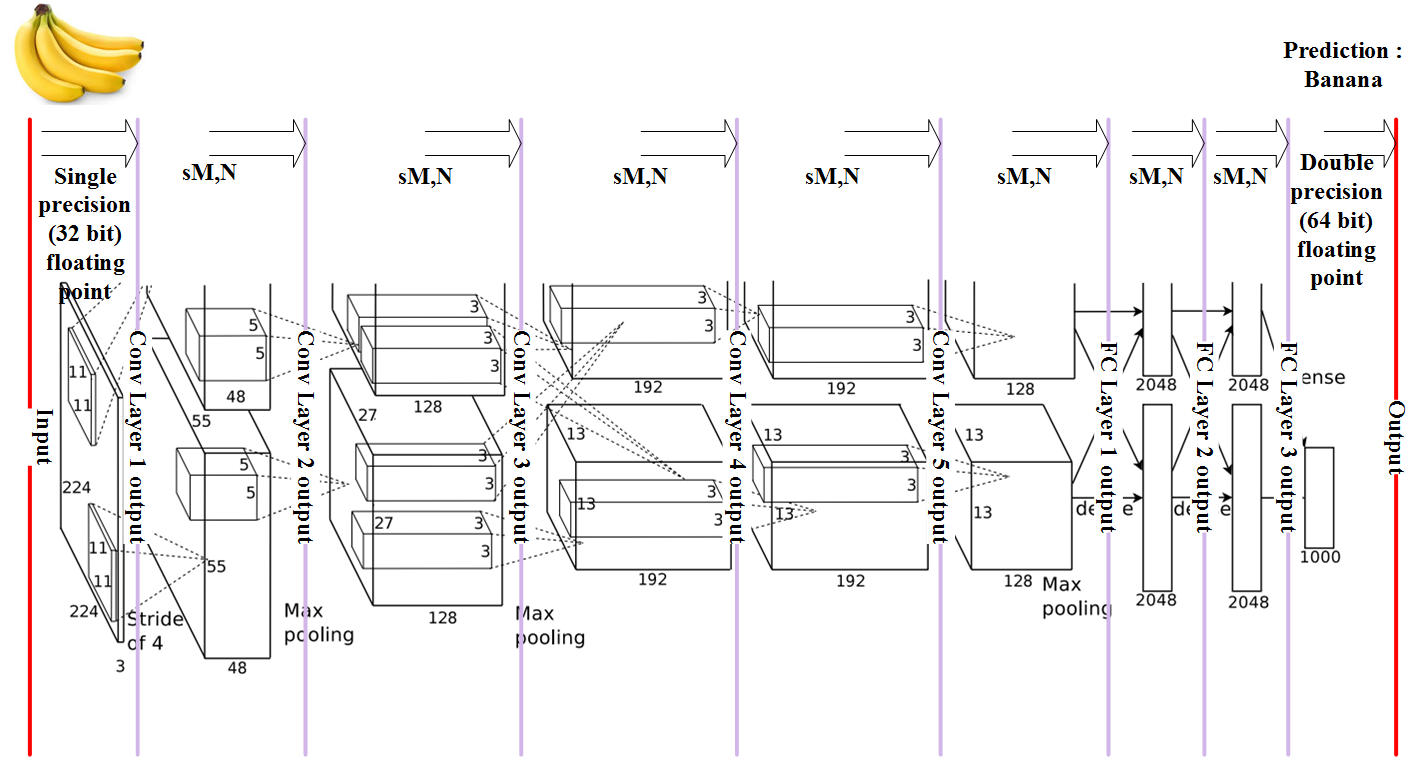
\includegraphics[width=3.5in]{fixedpt}
\caption{Forward Path of AlexNet with fixed precision sM,N}
\label{fp}
\end{figure}




\section{Results}
The Tables \ref{res1},\ref{res2},\ref{res3} and \ref{res4} show in detail the results of our analysis. They describe the prediction status (TRUE/FALSE) and the softmax score. Tables \ref{res1} and \ref{res2} show the result from AlexNet and Tables \ref{res3} and \ref{res4} show the results from VGGNET16. In both sets of results we can see the deterioration of the softmax score as the bit precision goes down. 


%The Tables \ref{res1},\ref{res2},\ref{res3} \ref{res4} below gives the prediction status (TRUE/FALSE) and the softmax score along with the software execution time of the entire network. The software execution time  also shows a declining trend as the number of bits in the fixed point precision are lowered. The software execution is much better for baseline precisions. This analysis shows that we can get away with using a lower fixed point precision for intermediate fmaps and not suffer in accuracy and be comparable to floating point operations.  

In Table \ref{res1} we compare the results achieved using fixed point precision with a single precision (32 bit) floating point. For this setup the input and filter weights are of s32,22 fixed point precision. We can see here that the forward pass of the network is able to correctly identify the input image of a banana however, its confidence scores keeps deteriorating with the smaller precisions. We see a good perfromance up until fixed point precision s12,4. The softmax score seems be very large for a correct predicion for s12,4. Changing the fractional length of the fixed point also has an effect on the softmax score as s12,5 performs poorly compared to s12,4. The softmax score keeps declining after s12,4 and we make a wrong prediction at s6,2.  
In Table \ref{res2} the input and the weights are s16,7 and we compare various fixed point precisions with the single precision performance. Here the softmax score is high and begins deteriorating after s12,4.

\begin{table}[!ht]
\centering
\caption{AlexNET:Results for fixed point precision quantization on output fmaps input and weights (s32,22), output double precision}
\label{res1}
\begin{tabular}{ccc}
\hline
                   & \textbf{Prediction}   & \textbf{softmax}  \\
\textbf{Precision} & \textbf{(True/False)} & \textbf{score}         \\ \hline
\color{red}\textbf{single}    & \color{red}TRUE                  & \color{red}9.80E-01          \\
\textbf{s32,22}    & TRUE                  & 9.82E-01                    \\
\textbf{s26,7}     & TRUE                  & 9.82E-01                    \\
\textbf{s16,7}     & TRUE                  & 9.82E-01                    \\
\textbf{s12,4}     & TRUE                  & 9.97E-01                      \\
\textbf{s12,5}     & TRUE                  & 6.68E-01                     \\
\textbf{s12,6}     & TRUE                  & 1.01E-01                     \\
\textbf{s10,4}     & TRUE                  & 1.01E-01                     \\
\textbf{s8,2}      & TRUE                  & 1.00E-01                     \\
\textbf{s6,2}      & FALSE                 & 2.77E-01                     \\ \hline
\end{tabular}
\end{table}


 


\begin{table}[!ht]
\centering
\caption{AlexNET:Results for fixed point precision quantization on output fmaps input and weights (s16,7), output double precision}
\label{res2}
\begin{tabular}{ccc}
\hline
                   & \textbf{Prediction} & \textbf{softmax}  \\ 
\textbf{Precision} & \textbf{(True/False)}    & \textbf{score}  \\ \hline
\color{red}\textbf{single}    & \color{red}TRUE                  & \color{red}9.80E-01         \\
\textbf{s16,7}     & TRUE                & 9.93E-01                     \\
\textbf{s12,4}     & TRUE                & 9.87E-01                     \\
\textbf{s10,4}     & TRUE                & 1.01E-01                      \\
\textbf{s8,2}      & TRUE                & 1.20E-01                    \\
\textbf{s6,2}      & FALSE               & 2.57E-02                     \\ \hline
\end{tabular}
\end{table}

In Table \ref{res3}, the input and filter weights are s45,17 fixed point precision. The result of all the fixed point precisions are compared against a double precision performance. 
Table \ref{res4} has input and filter weights set to s24,10 precision. It shows similar result from fixed point precisions compared against double precision. 
The softmax score in both Tables \ref{res3} and \ref{res4} deteriorates after s12,4 precision. 

\begin{table}[!ht]
\centering
\caption{VGGNET16:Results for fixed point precision quantization on output fmaps input and weights (s45,7), output double precision}
\label{res3}
\begin{tabular}{cccc}
\hline
                   & \textbf{Prediction} & \textbf{softmax}  \\
\textbf{Precision} & \textbf{(True/False)} & \textbf{score}         \\ \hline
\color{red}\textbf{double}    & \color{red}TRUE                & \color{red}9.57E-01                    \\
\textbf{s45,17}     & TRUE                & 9.57E-01          \\
\textbf{s32,12}    & TRUE                & 9.57E-01          \\
\textbf{s24,10}    & TRUE                & 9.44E-01          \\
\textbf{s16,6}     & FALSE               & 1.26E-01          \\ \hline
\end{tabular}
\end{table}

\begin{table}[!ht]
\centering
\caption{VGGNET16:Results for fixed point precision quantization on output fmaps input and weights (s24,10), output double precision}
\label{res4}
\begin{tabular}{cccc}
\hline
                   & \textbf{Prediction}   & \textbf{softmax}  \\ 
\textbf{Precision} & \textbf{(True/False)} & \textbf{score}           \\ \hline
\color{red}\textbf{double}    &\color{red} TRUE                  & \color{red}9.57E-01                     \\
\textbf{s24,10}    & TRUE                  & 9.59E-01        \\
\textbf{s16,6}     & FALSE                 & 1.23E+00          \\ \hline
\end{tabular}
\end{table}



%\begin{table*}[h!t]
%\centering
%\caption{AlexNET:Results for fixed point precision quantization on output fmaps input and weights (s32,22), output double precision}
%\label{res1}
%\begin{tabular}{ccccccccccc}
%\hline
%\textbf{}          & \textbf{Prediction}   & \textbf{softmax} & \textbf{conv1} & \textbf{conv2} & \textbf{conv3} & \textbf{conv4} & \textbf{conv5} & \textbf{fc1} & \textbf{fc2} & \textbf{fc3} \\ 
%
%\textbf{Precision} & \textbf{(True/False)} & \textbf{score}   & \textbf{sec}   & \textbf{sec}   & \textbf{sec}   & \textbf{sec}   & \textbf{sec}   & \textbf{sec} & \textbf{sec} & \textbf{sec} \\ \hline
%\textbf{s32,22}    & TRUE                  & 9.82E-01         & 15.433         & 20.306         & 12.0627        & 9.539          & 11.205         & 21.001       & 10.295       & 4.084        \\
%\textbf{s26,7}     & TRUE                  & 9.82E-01         & 15.595         & 10.113         & 12.552         & 4.9            & 6.717          & 17.475       & 8.781        & 4.281        \\
%\textbf{s16,7}     & TRUE                  & 9.82E-01         & 10.649         & 8.814          & 4.9            & 4.324          & 5.364          & 13.777       & 7.17         & 3.134        \\
%\textbf{s12,4}     & TRUE                  & 9.97E-01         & 10.559         & 9.314          & 5.1            & 5.013          & 5.641          & 13.95        & 7.534        & 3.474        \\
%\textbf{s12,5}     & TRUE                  & 6.68E-01         & 10.732         & 9.134          & 5.233          & 4.419          & 5.649          & 14.031       & 7.489        & 3.607        \\
%\textbf{s12,6}     & TRUE                  & 1.01E-01         & 10.38          & 8.63           & 5.093          & 4.327          & 5.686          & 13.944       & 7.171        & 3.394        \\
%\textbf{s10,4}     & TRUE                  & 1.01E-01         & 10.494         & 8.662          & 5.061          & 4.43           & 5.824          & 14.173       & 7.97         & 3.534        \\
%\textbf{s8,2}      & TRUE                  & 1.00E-01         & 10.492         & 8.923          & 5.163          & 4.64           & 5.885          & 14.152       & 7.272        & 3.461     \\
%\textbf{s6,2}      & FALSE                  & 2.77E-01         & 13.226        & 9.91 			& 5.661         & 4.27           & 6.162          & 14.631      & 7.867        & 3.6    \\ \hline
%\end{tabular}
%\end{table*}
%
%
%\begin{table*}[h!t]
%\centering
%\caption{AlexNET:Results for fixed point precision quantization on output fmaps input and weights (s16,7), output double precision}
%\label{res2}
%\begin{tabular}{ccccccccccc}
%\hline
%                   & \textbf{Prediction}   & \textbf{softmax} & \textbf{conv1} & \textbf{conv2} & \textbf{conv3} & \textbf{conv4} & \textbf{conv5} & \textbf{fc1} & \textbf{fc2} & \textbf{fc3} \\ 
%                   
%\textbf{Precision} & \textbf{(True/False)} & \textbf{score}   & \textbf{sec}   & \textbf{sec}   & \textbf{sec}   & \textbf{sec}   & \textbf{sec}   & \textbf{sec} & \textbf{sec} & \textbf{sec} \\ \hline
%\textbf{s16,7}     & TRUE                  & 9.93E-01         & 12.134         & 10.981         & 5.97           & 6.338          & 8.664          & 11.45        & 7.532        & 4            \\
%\textbf{s12,4}     & TRUE                  & 9.87E-01         & 12.389         & 10.189         & 5.642          & 5.0611         & 6.381          & 11.508       & 6.991        & 3.701        \\
%\textbf{s10,4}     & TRUE                  & 1.01E-01         & 11.005         & 10.125         & 5.735          & 5.09           & 6.516          & 11.569       & 6.908        & 3.676        \\
%\textbf{s8,2}      & TRUE                  & 1.20E-01         & 11.113         & 10.682         & 5.646          & 5.088          & 6.516          & 11.811       & 7.066        & 3.652        \\
%\textbf{s6,2}      & FALSE                 & 2.57E-02         & 14.731         & 10.672         & 5.6            & 5.022          & 6.79           & 12.222       & 7.029        & 3.628        \\ \hline
%\end{tabular}
%\end{table*}
%
%
%\begin{table*}[]
%\centering
%\caption{AlexNET:Results for fixed point precision quantization on output fmaps input and weights (s8,2), output double precision}
%\label{res3}
%\begin{tabular}{ccccccccccc}
%\hline
%                   & \textbf{Prediction} & \textbf{softmax} & \textbf{conv1} & \textbf{conv2} & \textbf{conv3} & \textbf{conv4} & \textbf{conv5} & \textbf{fc1} & \textbf{fc2} & \textbf{fc3} \\ 
%                   
%\textbf{Precision} & \textbf{(True/False)}       & \textbf{score }           & \textbf{sec}            & \textbf{sec}            & \textbf{sec}            & \textbf{sec}            & \textbf{sec}            & \textbf{sec}          & \textbf{sec}         & \textbf{sec}          \\ \hline
%\textbf{s8,2}      & FALSE               & 1.63E-03         & 10.989         & 9.175          & 4.883          & 4.608          & 6.001          & 7.479        & 5.034        & 3.001        \\
%\textbf{s6,2}      & FALSE               & 1.63E-03         & 11.478         & 9.039          & 4.769          & 4.449          & 5.18           & 7.716        & 4.804        & 3.08         \\ \hline
%\end{tabular}
%\end{table*}



%\subsubsection{FMap Selector}
%So many weights, 
%
%DeepCompression.
%
%
%
%
%Processing in Memory techniques. 


% no \IEEEPARstart


% You must have at least 2 lines in the paragraph with the drop letter
% (should never be an issue)


%\hfill mds
% 
%\hfill August 26, 2015



% Please add the following required packages to your document preamble:






% An example of a floating figure using the graphicx package.
% Note that \label must occur AFTER (or within) \caption.
% For figures, \caption should occur after the \includegraphics.
% Note that IEEEtran v1.7 and later has special internal code that
% is designed to preserve the operation of \label within \caption
% even when the captionsoff option is in effect. However, because
% of issues like this, it may be the safest practice to put all your
% \label just after \caption rather than within \caption{}.
%
% Reminder: the "draftcls" or "draftclsnofoot", not "draft", class
% option should be used if it is desired that the figures are to be
% displayed while in draft mode.
%
%\begin{figure}[!t]
%\centering
%\includegraphics[width=2.5in]{myfigure}
% where an .eps filename suffix will be assumed under latex, 
% and a .pdf suffix will be assumed for pdflatex; or what has been declared
% via \DeclareGraphicsExtensions.
%\caption{Simulation results for the network.}
%\label{fig_sim}
%\end{figure}

% Note that the IEEE typically puts floats only at the top, even when this
% results in a large percentage of a column being occupied by floats.


% An example of a double column floating figure using two subfigures.
% (The subfig.sty package must be loaded for this to work.)
% The subfigure \label commands are set within each subfloat command,
% and the \label for the overall figure must come after \caption.
% \hfil is used as a separator to get equal spacing.
% Watch out that the combined width of all the subfigures on a 
% line do not exceed the text width or a line break will occur.
%
%\begin{figure*}[!t]
%\centering
%\subfloat[Case I]{\includegraphics[width=2.5in]{box}%
%\label{fig_first_case}}
%\hfil
%\subfloat[Case II]{\includegraphics[width=2.5in]{box}%
%\label{fig_second_case}}
%\caption{Simulation results for the network.}
%\label{fig_sim}
%\end{figure*}
%
% Note that often IEEE papers with subfigures do not employ subfigure
% captions (using the optional argument to \subfloat[]), but instead will
% reference/describe all of them (a), (b), etc., within the main caption.
% Be aware that for subfig.sty to generate the (a), (b), etc., subfigure
% labels, the optional argument to \subfloat must be present. If a
% subcaption is not desired, just leave its contents blank,
% e.g., \subfloat[].


% An example of a floating table. Note that, for IEEE style tables, the
% \caption command should come BEFORE the table and, given that table
% captions serve much like titles, are usually capitalized except for words
% such as a, an, and, as, at, but, by, for, in, nor, of, on, or, the, to
% and up, which are usually not capitalized unless they are the first or
% last word of the caption. Table text will default to \footnotesize as
% the IEEE normally uses this smaller font for tables.
% The \label must come after \caption as always.
%
%\begin{table}[!t]
%% increase table row spacing, adjust to taste
%\renewcommand{\arraystretch}{1.3}
% if using array.sty, it might be a good idea to tweak the value of
% \extrarowheight as needed to properly center the text within the cells
%\caption{An Example of a Table}
%\label{table_example}
%\centering
%% Some packages, such as MDW tools, offer better commands for making tables
%% than the plain LaTeX2e tabular which is used here.
%\begin{tabular}{|c||c|}
%\hline
%One & Two\\
%\hline
%Three & Four\\
%\hline
%\end{tabular}
%\end{table}


% Note that the IEEE does not put floats in the very first column
% - or typically anywhere on the first page for that matter. Also,
% in-text middle ("here") positioning is typically not used, but it
% is allowed and encouraged for Computer Society conferences (but
% not Computer Society journals). Most IEEE journals/conferences use
% top floats exclusively. 
% Note that, LaTeX2e, unlike IEEE journals/conferences, places
% footnotes above bottom floats. This can be corrected via the
% \fnbelowfloat command of the stfloats package.


\section{Conclusion}
In this paper we learned that fixed point casting and arithmetic applied to output fmaps has an affect on the softmax score of the CNN. Thus, it will affect the accuracy of the output in test runs. However, we can afford to use lower precision before we see any substantial reduction in the softmax score. We have learned that the softmax score is also sensitive to the word length and fractional length of the output fmaps. Hence we need to pick them with care. It has confirmed our hypothesis and we can now choose the correct precision which can be substantially lower than the input and weight precisions. The performance of a double precision AlexNet forward pass is comparable to a s12,4 fixed point Alexnet forward pass. Similarly the performance of a double precision floating point VGGNET16 forward pass is comparable to a s12,4 fixed point VGGNET16 forward pass.
This analysis was done on dense networks and may lead to more saving on sparse networks. This work can be extended to other networks  such as ResidualNet , GoogleNet. We can also design a tool that will recommend the best fixed point precision. This technique can be combined with other techniques such as data reuse to design better hardware. 

% trigger a \newpage just before the given reference
% number - used to balance the columns on the last page
% adjust value as needed - may need to be readjusted if
% the document is modified later
%\IEEEtriggeratref{8}
% The "triggered" command can be changed if desired:
%\IEEEtriggercmd{\enlargethispage{-5in}}

% references section

% can use a bibliography generated by BibTeX as a .bbl file
% BibTeX documentation can be easily obtained at:
% http://mirror.ctan.org/biblio/bibtex/contrib/doc/
% The IEEEtran BibTeX style support page is at:
% http://www.michaelshell.org/tex/ieeetran/bibtex/
\bibliographystyle{IEEEtran}
% argument is your BibTeX string definitions and bibliography database(s)
\bibliography{IEEEabrv,references_1}
%
% <OR> manually copy in the resultant .bbl file
% set second argument of \begin to the number of references
% (used to reserve space for the reference number labels box)
%\begin{thebibliography}{1}
%
%\bibitem{IEEEhowto:kopka}
%H.~Kopka and P.~W. Daly, \emph{A Guide to \LaTeX}, 3rd~ed.\hskip 1em plus
%  0.5em minus 0.4em\relax Harlow, England: Addison-Wesley, 1999.
%
%\end{thebibliography}




% that's all folks
\end{document}


